\documentclass[svgnames]{report}
\usepackage[left = 2.75cm,right =2.75cm,top=3cm,bottom=3cm]{geometry}
\usepackage{graphicx}
\usepackage{tikz}
\usepackage[T1]{fontenc}
\usepackage[utf8]{inputenc}
\usepackage[french]{babel}
\usepackage{subcaption}
\usepackage{caption}
\usepackage{color}
\usepackage[final]{listings}
\lstset{
    basicstyle=\ttfamily\color{green!50!blue}
}

\lstdefinestyle{python}{
    language=Python,
}

\usepackage[explicit]{titlesec}



\frenchbsetup{StandardLists=true} % à inclure si on utilise \usepackage[french]{babel}
\usepackage{enumitem}
\renewcommand{\thefigure}{\arabic{figure}}
\titlespacing*{\chapter}{0pt}{-10pt}{30pt}


\usepackage{hyperref} % Créer des liens et des signets 
\hypersetup{
colorlinks = true, %colorise les liens
breaklinks = true, %permet le retour à la ligne dans les liens trop long
urlcolor = blue, %couleur des hyperliens
linkcolor = blue, %couleur des liens internes
citecolor = black, %couleur des références
frenchlinks = true
} 


\newcommand*\chapterlabel{}
\titleformat{\chapter}
  {\gdef\chapterlabel{}
   \normalfont\sffamily\Huge\bfseries}
  {\gdef\chapterlabel{Partie \thechapter\ --\ }}{0pt}
      {\begin{tikzpicture}[remember picture, overlay]
       \node[right=-0.5cm,rectangle,rounded corners=5pt,fill=brown!15]{\color{black}\chapterlabel#1};
  \end{tikzpicture}
 }

\newcommand*\sectionlabel{}
\titleformat{\section}
  {\gdef\sectionlabel{}
   \normalfont\sffamily\Large\bfseries}
  {\gdef\sectionlabel{\thesection\ --\ }}{0pt}
      {\begin{tikzpicture}[remember picture, overlay]
       \node[right=-0.25cm,rectangle,rounded corners=5pt,fill=brown!15]{\color{black}\sectionlabel#1};
  \end{tikzpicture}
 }

\newcommand*\subsectionlabel{}
\titleformat{\subsection}
  {\gdef\subsectionlabel{}
   \normalfont\sffamily\bfseries}
  {\gdef\subsectionlabel{\thesubsection\ --\ }}{0pt}
      {\begin{tikzpicture}[remember picture, overlay]
       \node[right,rectangle,rounded corners=5pt,fill=brown!15]{\color{black}\subsectionlabel#1};
  \end{tikzpicture}
 }

\newcommand*\subsubsectionlabel{}
\titleformat{\subsubsection}
  {\gdef\subsubsectionlabel{}
   \normalfont\sffamily\bfseries}
  {\gdef\subsubsectionlabel{}}{0pt}
      {\begin{tikzpicture}[remember picture, overlay]
       \node[right=0.25cm,rectangle,rounded corners=5pt,fill=brown!15]{\color{black}#1};
  \end{tikzpicture}
 }

\usepackage{fancyhdr}
\pagestyle{fancy}




\renewcommand{\chaptermark}[1]{\markboth{\bsc{\chaptername~\thechapter{} :} #1}{}}

\renewcommand\headrulewidth{1pt}

\fancyhead[R]{\scriptsize\large 12/02/2024}
\fancyhead[L]{\scriptsize\large \leftmark}

\renewcommand\footrulewidth{1pt}
\fancyfoot[R]{\scriptsize\large Méthode de calcul/Limite de la machine}
\fancyfoot[C]{\thepage}

\begin{document}
\begin{titlepage} % Suppresses displaying the page number on the title page and the subsequent page counts as page 1
	
	\colorbox{brown!15}{
		\parbox[t]{0.93\textwidth}{ % Outer full width box
			\parbox[t]{0.91\textwidth}{ % Inner box for inner right text margin
				\raggedleft % Right align the text
				\vspace{0.7cm} % Space between the start of the title and the top of the grey box
                                {\sffamily\Huge\bfseries
                                \textbf{Méthode de calcul numérique}}
                                
                                \vspace{0.5cm}
                                
                                {\Huge Limites de la machine}\\
                                \vspace{0.3cm}
                                \Large
                                Rapport de projet\\
                                \vspace{0.3cm}
                                \vspace{0.3cm}
                                \Large
                                12/02/2024
				\vspace{0.7cm} % Space between the end of the title and the bottom of the grey box
			}
		}
	}

	\vfill % Space between the title box and author information
        
        \hfill
        \begin{minipage}{.55\textwidth}%
          \parbox[t]{0.93\textwidth}{ % Box to inset this section slightly
            \raggedleft % Right align the text
            \large % Increase the font size
            
            
\includegraphics[scale=0.4]{LogoENSEIRB.png}
          }
          
        \end{minipage}
	
\end{titlepage}
            
\setcounter{page}{1}


\tableofcontents

\subsection*{Résumé}
Le but principal de ce premier projet d'algorithmes numériques est d'appréhender la représentation des nombres en machines avec la partie 1. La deuxième partie a pour objectif quant à elle de comparer des erreurs avec des applications sur des fonctions qui sont l'algorithme népérien d'une part et ceux de CORDIC de l'autre.

\chapter{Partie 1}
\section{Objectif de la partie}
Comme énoncé dans le résumé introductif de la page précédente, cette partie va se concentrer sur la représentation de nombres décimaux réduits ainsi que leur utilisation pour pouvoir comparer des erreurs relatives lors de la manipulation de ces nombres tronqués.

\section{Créer la représentation et évaluer les erreurs relatives}
\subsubsection{Représentation décimale réduite}
Étapes prises durant la création de l'algorithme : 
\begin{itemize}
    \item conversion du nombre en une chaine de caractères str\_x;
    \item stockage du signe dans s;
    \item stockage du nombre de zéros après la virgule dans num\_zeros;
    \item stockage de la partie significative en new\_x selon l'algorithme suivant :
    \noindent\begin{lstlisting}[frame=single,style=python]
new_x <- 0
pour i allant de db_partie_significative a fn_partie_significative
debut
    new_x <- new_x + str_x[i] x 10
fin
    \end{lstlisting}
    
    \item arrondi au supérieur de la partie significative;
    \item rajout des zéros de l'après partie significative à num\_zeros si la virgule n'a pas encore été touché;
    \item récupération du résultat final en calculant : $s\times{new\_x}\times{10^{num\_zeros}}$
\end{itemize}


\subsubsection{Erreur relative : la somme et le produit}
\noindent Pour cette fonction représentant $\delta_s$, nous avons utilisé la fonction précédente pour créer x et y en "machine" (c'est à dire leur représentation réduite) ainsi que leur somme en "machine". 

Cette étape préalable permet que la somme de x et y "machine" simule bien la représentation de la somme dans une machine volontairement peu précise. Une fois ceci fait il suffit de calculer le delta avec le x et y donnés à la fonction.

\noindent\begin{lstlisting}[frame=single,style=python]
def delta_somme(x,y,p):
    x_machine = rp(x,p)
    y_machine = rp(y,p)
    return abs(x+y - rp((x_machine + y_machine),p))/abs(x+y)
\end{lstlisting}

\noindent De la même manière pour la multiplication , il suffit de séparer les calculs en "machine" et les calculs supposés réels avec une fonction identique à ci dessus mais en remplaçant la somme par le produit de compléxité similaire à la précédente.

\subsection{Tests de la représentation décimale et comparaison d'erreur relative selon la précision}

Pour cette partie nous avons tester sur plusieurs valeurs la fonction rp dont celles présentées dans le fascicule de TD.

\begin{center}
\noindent \begin{tabular}{|l|l|l|}
  \hline
  Nombre réel & Sur 4 décimales & Sur 6 décimales\\ \hline
  3.141592658 & 3.142 & 3.1415900000000003\\
  10507.1823 & 10510 & 10507.2 \\
  0.0001857563 & 0.0001858 & 0.000185756 \\
  \hline
\end{tabular}
\end{center}

\begin{figure}[h]
    \centering
    \begin{subfigure}{0.4\textwidth}
        \centering
        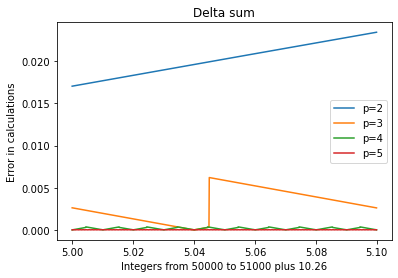
\includegraphics[width=1\linewidth]{Delta_sum.png}
        \caption{Addition}
        \label{fig:Delta_sum}
    \end{subfigure}
    \begin{subfigure}{0.4\textwidth}
        \centering
        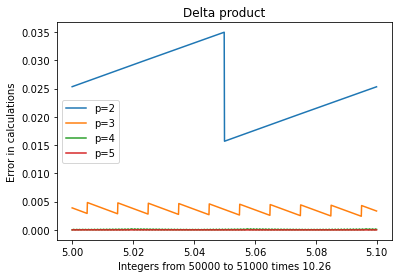
\includegraphics[width=1\linewidth]{Delta_product.png}
        \caption{Multiplication}
        \label{fig:Delta_prod}
    \end{subfigure}
    \caption{Comparaison d'erreurs machines dans les opérations binaires}
    \label{fig:Delta_binop}
\end{figure}

Les valeurs étudiées mettent en évidence des cycles dans les marges d'erreurs de la machine pour différentes précisions, avec des courbes régulières en dent de scie. En prenant en compte le fait que la figure \ref{fig:Delta_sum} présente les courbes de valeurs sur un interval plus petit que la figure \ref{fig:Delta_prod}, on retrouve des cycles similaires pour une même précision entre l'addition et la multiplication. De plus, plus la précision p est grande, plus la marge d'erreur reste proche de 0.\\

Ces cycles sont explicables par l'arrondissement des valeurs pour respecter les limites de la précision : pour une précision de 3, les valeurs 1.185 et 1.194 seront toutes les deux lues comme 1.19. Ces erreurs d'imprécision s'accumulent jusqu'à atteindre la valeur arrondie suivante ; une précision p plus grande permet d'atteindre cette valeur plus rapidement, et donc d'avoir une plus petite marge d'erreur.\\

\chapter{Partie 2}
\section{Algorithmes de CORDIC}

\subsection{Précision et approximation de calcul}

En dehors des erreurs dues à la représentation en mémoire des valeurs, une imprécision dans les calculs peut être un effet secondaire d'une optimisation du reste du programme. Nous regardons ici le cas du calcul du logarithme népérien de 2 utilisant une approximation de la valeur :

\[log(2) = \sum_{n=0}^{\infty}\frac{(-1)^{n+1}}{n}\]

Une somme à l'infinie n'est pas possible dans une application concrète du calcul, le résultat ne pourra donc être qu'une approximation de ln(2) ; mais le calcul même ne demande pas une machine puissante.

\subsection{Cas de la calculatrice}
Le cas de la calculatrice est un bon exemple de l'utilisation et de l'importance des algorithmes de CORDIC. En effet, les ressources étant limités (puissance de calcul, mémoire) il faut réussir à donner des résultats précis en limitant au maximum les erreurs d'approximations et dans un temps assez court pour satisfaire l'utilisateur.

La représentation des nombres dans une calculatrice est la suivante : 
\begin{itemize}
    \item Un nombre 'flottant' sur 8 octets
    \item Une mantisse constituée de 13 chiffres codés indépendant sur 4 chiffres binaires
    \item Un exposant 
    \item Le signe du nombre (et de l'exposant s'il n'est pas signé) 
\end{itemize}
Cette représentation des nombres possède des avantages et des défauts : 
\begin{itemize}
    \item Avantages : 
    \begin{enumerate}
        \item Rapidité d'exécution des calculs grace à une taille de nombre raisonable et une méthode de résolution par décalage de bits
        \item Une précision relative pour les réels satisfaisante
    \end{enumerate}
    \item{Défauts} 
    \begin{enumerate}
        \item Perte de précision pour les petits nombres, engendre des erreurs de plus en plus grande lors des calculs précis à cause de l'arrondissement des valeurs 
    \end{enumerate}
\end{itemize}
\subsection{Calcul des fonctions usuelles}
La fin du projet s'intéresse à l'implémentation de 4 algorithmes pour calculer fonctions trigonométriques et exponentielle. \newline 
Ces 4 algorithmes reposent sur le principe d'éviter les multiplications et les divisions pour les calculs car ce sont des opérations lourdes sur une calculatrice. Afin d'éviter les opérations lourdes, les algorithmes fonctionnent de la manière suivante :
\begin{itemize}
    \item \textbf{Réduction de la valeur d'entrée dans un intervalle approprié} : Pour les fonctions comme ln et exp, la valeur d'entrée est réduite à un intervalle où les méthodes de calcul sont efficaces. Par exemple, pour ln, la valeur est ramenée à l'intervalle [1, 10[.
    \item \textbf{Application de l'algorithme CORDIC} : Une fois que la valeur d'entrée est dans l'intervalle approprié, l'algorithme CORDIC est appliqué en itérant sur un ensemble précalculé de valeurs. Ces valeurs sont utilisées pour effectuer des transformations simples telles que l'addition, la soustraction et le décalage de bits (peu couteuse en machine).
    Chaque fonction suit des transformations différentes pour réduire l'entrée tout en calculant le résultat.
    \item \textbf{Interpolation linéaire pour précision supplémentaire} : Une fois les transformations appliquées, le résultat final est obtenu par interpolation linéaire ou par d'autres méthodes d'approximation pour obtenir une précision supplémentaire si nécessaire.
\end{itemize}

Les résultats obtenus sont corrects en deçà d'une certaine précision.

\vspace{0.5cm}
\begin{figure}[h]
    \centering
    \begin{subfigure}{0.3\textwidth}
        \centering
        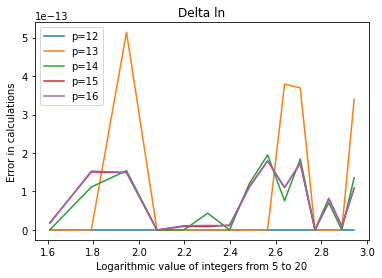
\includegraphics[width=1\linewidth]{Delta_ln.png}
        \caption{Logarithme néperien}
        \label{fig:Delta_ln}
    \end{subfigure}
    \begin{subfigure}{0.3\textwidth}
        \centering
        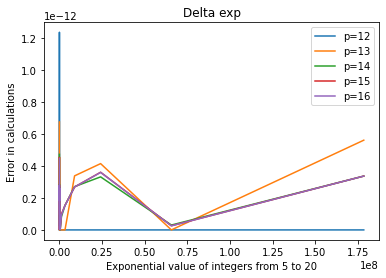
\includegraphics[width=1\linewidth]{Delta_exp.png}
        \caption{Exponentiel}
        \label{fig:Delta_exp}
    \end{subfigure}
    \begin{subfigure}{0.3\textwidth}
        \centering
        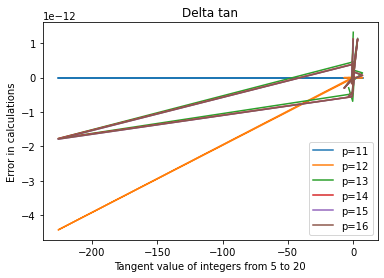
\includegraphics[width=1\linewidth]{Delta_tan.png}
        \caption{Tangeante}
        \label{fig:Delta_tan}
    \end{subfigure}
    \begin{subfigure}{0.3\textwidth}
        \centering
        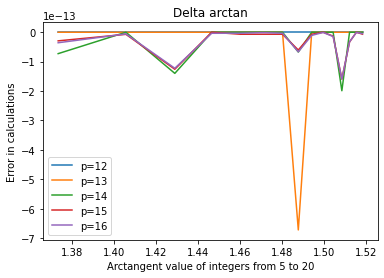
\includegraphics[width=1\linewidth]{Delta_atan.png}
        \caption{Arctangeante}
        \label{fig:Delta_atan}
    \end{subfigure}
    \caption{Comparaison d'erreurs machines dans les algorithmes CORDICs}
    \label{fig:Delta_cordic}
\end{figure}

Dans les applications des algorithmes CORDIC pour le logarithme, l'exponentielle, la tangeante et l'arctangeante, on observe des valeurs très aléatoires dans les marges d'erreurs qui ne sont pas corrélées à la valeur de la précision. Puisque ces calculs sont basés sur une approximation des valeurs recherchées, une plus petite précision dans les valeurs est préférable : ainsi on constate que les erreurs ne deviennent visibles qu'à partir d'une précision de douze chiffres.\\

Cette technique permet d'obtenir des résultats rapidement car la valeur d'entrée est réduite jusqu'à des valeurs ou les calculs peuvent être effectués efficacement. 

Dans le contexte d'une calculatrice, cette technique est pertinente car elle évite les calculs lourds (respecte la limite de puissance de calcul de la calculatrice) 
De plus, elle effectue le calcul de manière rapide, pour fournir un résultat pertinent et rapidement à l'utilisateur en respectant les contraintes technologiques de la calculatrice (faible puissance de calcul et faible mémoire)

\end{document}

